\begingroup
\renewcommand*{\arraystretch}{1.2}
\newcommand{\tmp}{\phantom{, 200}}
\begin{table}[!h]
  \topcaption{Summary of the nominal (\njet, \nb, \scalht, \mht)
    binning schema. Each entry (and the following entry, if present)
    signifies the lower (upper) bound of an \mht bin within a given
    (\njet, \nb, \scalht) bin. Unique or final entries represent \mht
    bins unbounded from above. A dash (--) signifies that the \scalht 
    bin in a given (\njet, \nb) category is not used in the analysis,
    in which case counts in high-\scalht bins are integrated into the
    adjacent lower-\scalht bin. For monojet events, $\scalht \equiv
    \mht$. The {\it a} denotes asymmetric \pt thresholds for the two
    highest \pt jets. 
  }
  \label{tab:binning}
  \centering
  \resizebox{\textwidth}{!}{
    \begin{tabular}{rrlllll}
      \hline
      \njet      & \nb       & \multicolumn{5}{c}{\scalht [GeV]}                                        \\ 
      \cline{3-7}
                 &           & 200 & 400      & 600           & 900                & 1200               \\
      \hline
      1          & 0         & 200 & 400 \tmp & 600 \tmp \tmp & 900 \tmp \tmp \tmp & --                 \\ 
      1          & 1         & 200 & 400 \tmp & 600 \tmp \tmp & --                 & --                 \\ 
      ${\geq}2a$ & 0         & 200 & 200, 400 & 200, 400, 600 & 200, 900 \tmp \tmp & --                 \\ 
      ${\geq}2a$ & 1         & 200 & 200, 400 & 200, 400, 600 & 200, 900 \tmp \tmp & --                 \\ 
      ${\geq}2a$ & 2         & 200 & 200, 400 & 200, 400, 600 & 200, 900 \tmp \tmp & --                 \\ 
      ${\geq}2a$ & ${\geq}3$ & 200 & 200, 400 & 200, 400, 600 & --                 & --                 \\ 
      2          & 0         & 200 & 200, 400 & 200, 400, 600 & 200, 400, 600, 900 & 200, 400, 600, 900 \\ 
      2          & 1         & 200 & 200, 400 & 200, 400, 600 & 200, 400, 600, 900 & 200, 400, 600, 900 \\ 
      2          & 2         & 200 & 200, 400 & 200, 400, 600 & --                 & --                 \\ 
      3          & 0         & 200 & 200, 400 & 200, 400, 600 & 200, 400, 600, 900 & 200, 400, 600, 900 \\ 
      3          & 1         & 200 & 200, 400 & 200, 400, 600 & 200, 400, 600, 900 & 200, 400, 600, 900 \\ 
      3          & 2         & 200 & 200, 400 & 200, 400, 600 & 200, 400, 600, 900 & 200, 400, 600, 900 \\ 
      3          & 3         & 200 & 200, 400 & 200, 400, 600 & --                 & --                 \\ 
      4          & 0         & --  & 200, 400 & 200, 400, 600 & 200, 400, 600, 900 & 200, 400, 600, 900 \\ 
      4          & 1         & --  & 200, 400 & 200, 400, 600 & 200, 400, 600, 900 & 200, 400, 600, 900 \\ 
      4          & 2         & --  & 200, 400 & 200, 400, 600 & 200, 400, 600, 900 & 200, 400, 600, 900 \\ 
      4          & ${\geq}3$ & --  & 200, 400 & 200, 400, 600 & 200, 400, 600, 900 & --                 \\ 
      5          & 0         & --  & 200, 400 & 200, 400, 600 & 200, 400, 600 \tmp & 200, 400, 600, 900 \\ 
      5          & 1         & --  & 200, 400 & 200, 400, 600 & 200, 400, 600 \tmp & 200, 400, 600, 900 \\ 
      5          & 2         & --  & 200, 400 & 200, 400, 600 & 200, 400, 600 \tmp & 200, 400, 600, 900 \\ 
      5          & 3         & --  & 200, 400 & 200, 400, 600 & 200, 400, 600 \tmp & --                 \\ 
      5          & ${\geq}4$ & --  & 200, 400 & --            & --                 & --                 \\ 
      ${\geq}6$  & 0         & --  & 200 \tmp & 200, 400 \tmp & 200, 400, 600 \tmp & 200, 400, 600, 900 \\ 
      ${\geq}6$  & 1         & --  & 200 \tmp & 200, 400 \tmp & 200, 400, 600 \tmp & 200, 400, 600, 900 \\ 
      ${\geq}6$  & 2         & --  & 200 \tmp & 200, 400 \tmp & 200, 400, 600 \tmp & 200, 400, 600, 900 \\ 
      ${\geq}6$  & 3         & --  & 200 \tmp & 200, 400 \tmp & 200, 400, 600 \tmp & 200, 400, 600, 900 \\ 
      ${\geq}6$  & ${\geq}4$ & --  & 200 \tmp & --            & --                 & --                 \\ 
      \hline
    \end{tabular}
  }
\end{table}
\endgroup

\begingroup
\renewcommand*{\arraystretch}{1.1}
\begin{table}[!t]
  \topcaption{Observed counts of candidate signal events and SM
    expectations determined from the CR-only fit using the simplified
    binning schema, as a function of \njet, \nb, and \mht. All counts
    are integrated over \scalht. The uncertainties include both
    statistical and systematic contributions. 
    The {\it a} denotes asymmetric \pt thresholds for the two highest \pt
    jets. 
  }
  \label{tab:simplified}
  \centering
  \begin{tabular}{rrlr@{}lr@{}lr@{}lr@{}l}
    \hline
    \njet           & \nb       &      & \multicolumn{8}{c}{\mht [GeV]}                                                                             \\
    \cline{4-11}
                    &           &      & 200        &                   & 400       &                & 600   &               & 900   &              \\
    \hline
%    =1, ${\geq}2a$  & 0         & Data & 411\,184   &                   & 11\,448   &                & 1116  &               & 111                  \\
%                    &           & SM   & $360\,000$ & $\,\pm\, 35\,000$ & $9990$    & $\,\pm\, 890$  & $910$ & $\,\pm\, 300$ & $107$ & $\,\pm\, 64$ \\[0.2ex]
%    =1, ${\geq}2a$  & ${\geq}1$ & Data & 31\,174    &                   & 769       &                & 96    &               & 16                   \\
%                    &           & SM   & $25\,500$  & $\,\pm\, 2300$    & $649$     & $\,\pm\, 61$   & $65$  & $\,\pm\, 20$  & $11$  & $.4 \pm 6.7$ \\[0.2ex]
%    =2, =3          & =0, =1    & Data & 66\,955    &                   & 5946      &                & 903   &               & 100                  \\
%                    &           & SM   & $58\,000$  & $\,\pm\, 10\,000$ & $5410$    & $\,\pm\, 970$  & $860$ & $\,\pm\, 330$ & $113$ & $\,\pm\, 76$ \\[0.2ex]
%    =2, =3          & ${\geq}2$ & Data & 1045       &                   & 70        &                & 6     &               & 0                    \\
%                    &           & SM   & $870$      & $\,\pm\, 130$     & $56$      & $.9 \pm 8.8$   & $7$   & $.1 \pm 2.6$  & $1$   & $.0 \pm 0.7$ \\[0.2ex]
%    =4, =5          & =0, =1    & Data & 9546       &                   & 1734      &                & 315   &               & 44                   \\
%                    &           & SM   & $10490$    & $\,\pm\, 1100$    & $1880$    & $\,\pm\, 250$  & $320$ & $\,\pm\, 110$ & $40$  & $\,\pm\, 27$ \\[0.2ex]
%    =4, =5          & ${\geq}2$ & Data & 1012       &                   & 93        &                & 4     &               & 3                    \\
%                    &           & SM   & $970$      & $\,\pm\, 120$     & $81$      & $.2 \pm 9.4$   & $8$   & $.4 \pm 2.4$  & $1$   & $.2 \pm 0.7$ \\[0.2ex]
%    ${\geq}6$       & =0, =1    & Data & 758        &                   & 141       &                & 33    &               & 5                    \\
%                    &           & SM   & $910$      & $\,\pm\, 180$     & $167$     & $\,\pm\, 71$   & $33$  & $\,\pm\, 25$  & $4$   & $.2 \pm 5.4$ \\[0.2ex]
%    ${\geq}6$       & ${\geq}2$ & Data & 197        &                   & 14        &                & 3     &               & 0                    \\
%                    &           & SM   & $189$      & $\,\pm\, 39$      & $16$      & $.9 \pm 4.8$   & $2$   & $.1 \pm 1.2$  & $0$   & $.2 \pm 0.3$ \\
    =1, ${\geq}2a$ & 0         & Data & 411\,184   &                   & 11\,448   &                & 1116  &               & 111                  \\
                   &           & SM   & $360\,000$ & $\,\pm\, 38\,000$ & $10\,000$ & $\,\pm\, 1400$ & $910$ & $\,\pm\, 170$ & $107$ & $\,\pm\, 28$ \\[0.2ex]
    =1, ${\geq}2a$ & ${\geq}1$ & Data & 31\,174    &                   & 769       &                & 105   &               & 7                    \\
                   &           & SM   & $25\,500$  & $\,\pm\, 2500$    & $649$     & $\,\pm\, 91$   & $69$  & $\,\pm\, 13$  & $6$   & $.4 \pm 1.8$ \\[0.2ex]
    =2, =3         & =0, =1    & Data & 66\,955    &                   & 5946      &                & 903   &               & 100                  \\
                   &           & SM   & $58\,000$  & $\,\pm\, 11\,000$ & $5400$    & $\,\pm\, 1100$ & $860$ & $\,\pm\, 220$ & $113$ & $\,\pm\, 41$ \\[0.2ex]
    =2, =3         & ${\geq}2$ & Data & 1045       &                   & 70        &                & 6     &               & 0                    \\
                   &           & SM   & $870$      & $\,\pm\, 130$     & $56$      & $.9 \pm 9.4$   & $7$   & $.1 \pm 1.7$  & $1$   & $.0 \pm 0.4$ \\[0.2ex]
    =4, =5         & =0, =1    & Data & 9546       &                   & 1734      &                & 315   &               & 44                   \\
                   &           & SM   & $10\,500$    & $\,\pm\, 1100$    & $1880$    & $\,\pm\, 310$  & $319$ & $\,\pm\, 71$  & $40$  & $\,\pm\, 14$ \\[0.2ex]
    =4, =5         & ${\geq}2$ & Data & 1012       &                   & 93        &                & 4     &               & 3                    \\
                   &           & SM   & $970$      & $\,\pm\, 110$     & $81$      & $\, \pm 11$    & $8$   & $.4 \pm 1.7$  & $1$   & $.2 \pm 0.4$ \\[0.2ex]
    ${\geq}6$      & =0, =1    & Data & 758        &                   & 141       &                & 33    &               & 5                    \\
                   &           & SM   & $910$      & $\,\pm\, 180$     & $167$     & $\,\pm\, 76$   & $33$  & $\,\pm\, 25$  & $4$   & $.2 \pm 5.0$ \\[0.2ex]
    ${\geq}6$      & ${\geq}2$ & Data & 197        &                   & 14        &                & 3     &               & 0                    \\
                   &           & SM   & $189$      & $\,\pm\, 40$      & $16$      & $.9 \pm 4.9$   & $2$   & $.1 \pm 1.2$  & $0$   & $.2 \pm 0.2$ \\
    \hline
  \end{tabular}
\end{table}
\endgroup

\begin{figure}[!b]
  \centering
  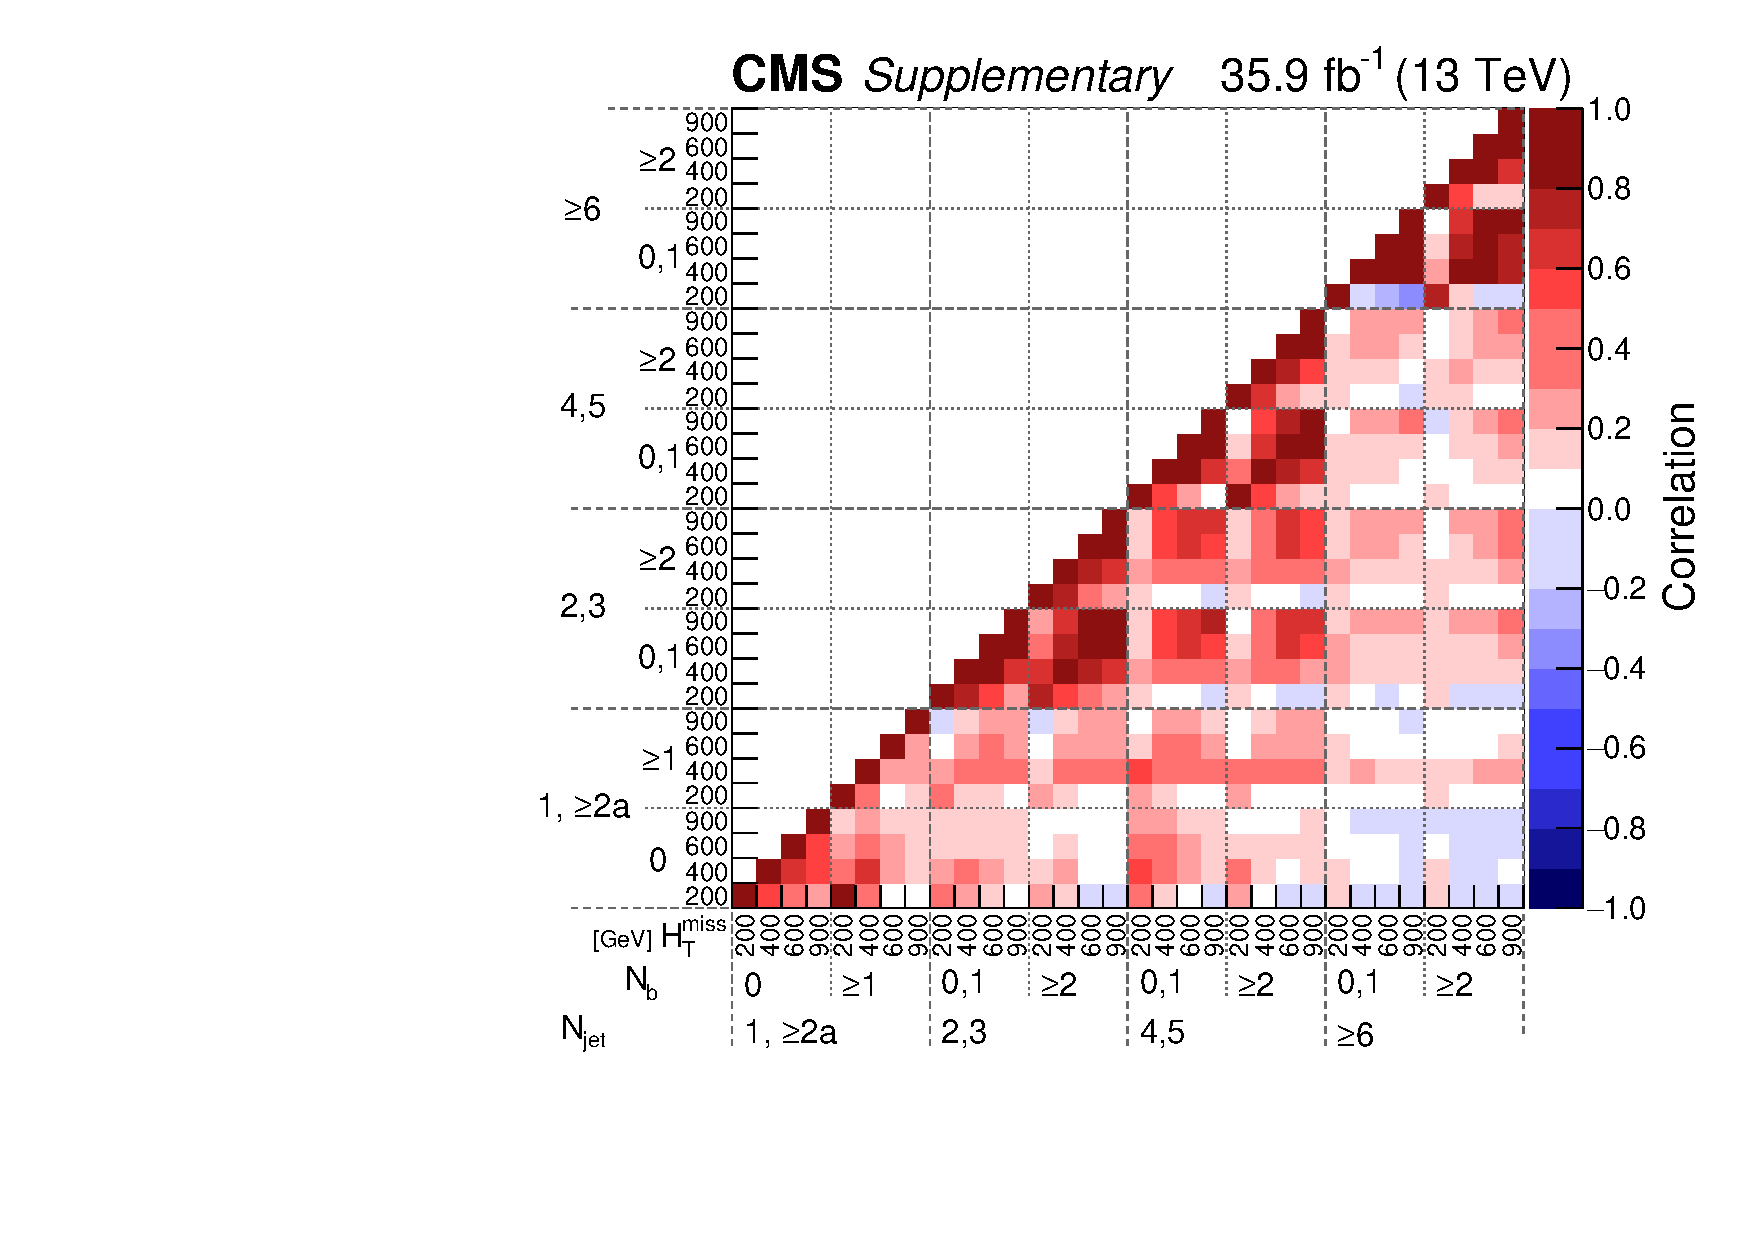
\includegraphics[width=0.6\textwidth]{Figures/correlation_supplementary.pdf}
  \caption{Correlation matrix for the SM background estimates
    determined from the CR-only fit using the simplified binning
    schema defined in Table~\ref{tab:simplified}.}
  \label{fig:correlation}
\end{figure} 
